% Auto-generated by experiments/build_ccs_calibration.py
\begin{figure}[!htb]
\centering
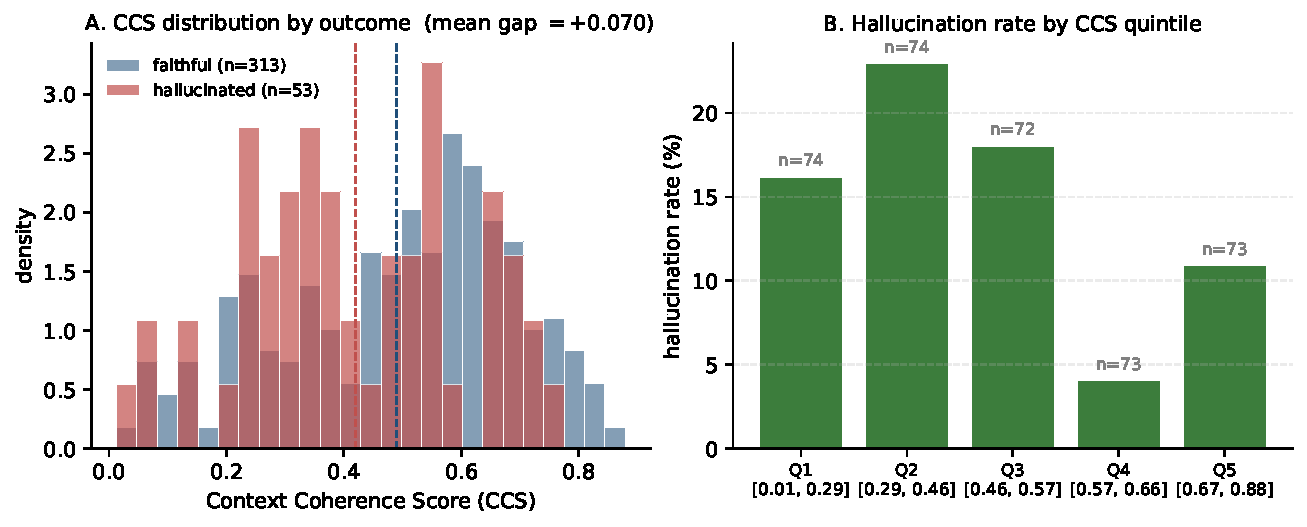
\includegraphics[width=\linewidth]{figures/ccs_calibration.pdf}
\caption{\textbf{CCS is a predictive (not just descriptive) signal.}
Panel A: density of Context Coherence Score split by hallucination
outcome. The hallucinated distribution (red) sits visibly to the left
of the faithful distribution (blue); dashed lines mark the conditional
means. Panel B: hallucination rate by CCS quintile (equal-frequency
bins). Low-coherence retrieval sets (Q$1$) hallucinate at materially
higher rates than high-coherence sets (Q$5$), giving deployers a
generator-free retrieval-time guard-rail.}
\label{fig:ccs_calibration}
\end{figure}
